\capitulo{5}{Aspectos relevantes del desarrollo del proyecto}

En este capítulo se expone de manera detallada el recorrido completo del proyecto, desde su concepción inicial hasta la evaluación de los resultados finales. Se narrará el proceso de investigación, las decisiones de diseño, los desafíos técnicos encontrados y las soluciones implementadas. El objetivo es ofrecer una visión transparente y cronológica de todo el trabajo realizado, explicando no solo el <<qué>> se ha hecho, sino también el <<porqué>> de cada paso. Se comenzará con la fase de exploración y prototipado, para luego profundizar en la creación del conjunto de datos propio, la optimización del modelo y el análisis de su rendimiento e interpretabilidad, culminando con el desarrollo de una aplicación web para su demostración.

\section{Pruebas iniciales y estado del arte}

La primera etapa del proyecto fue de carácter exploratorio. El objetivo era investigar el panorama actual del mundo de la ciberseguridad y cómo se podía aplicar la IA al mismo, validando dicha idea central y construyendo un prototipo inicial que sirviera como base y prueba de concepto para el resto del trabajo.

\subsection{Estado del arte y base del proyecto}

En sus orígenes, la idea principal de este proyecto era considerablemente más más abstracta y se centraba en un área distinta de la ciberseguridad. La intención inicial era explorar si las técnicas de inteligencia artificial (IA) podrían utilizarse para detectar o mitigar vulnerabilidades de \textit{hardware}, como los ataques de canal lateral (\textit{side-channel}) y de ejecución especulativa, del estilo de Spectre y Meltdown. Sin embargo, tras una primera investigación acerca de la literatura científica disponible, se determinó que este campo era extremadamente complejo y la cantidad de trabajos que aplicaban IA a este problema era muy escasa, concluyendo pues que, este enfoque habría sido demasiado ambicioso y un poco <<cogido con pinzas>>.

Esta falta de base sólida motivó un giro en la investigación hacia un área más consolidada: el análisis de \textit{malware}. Se estudiaron los diferentes enfoques de análisis (estático, dinámico e híbrido) y, de entre ellos, se determinó que el más interesante para indagar en el sería el análisis estático, principalmente debido a su principal ventaja: la capacidad de detectar \textit{malware} sin necesidad de ejecutar el software sospechoso, eliminando así prácticamente cualquier riesgo de infección para el sistema anfitrión. Cabe destacar que, aunque se consideró la idea de un enfoque híbrido, combinando una primera fase estática con un análisis dinámico guiado el cual se ejecutaría dentro de un entorno de \textit{sandbox}, la complejidad de implementar un sistema así excedía el alcance de este trabajo.

Por tanto, la idea del proyecto se estructuró en torno a la construcción de un clasificador de \textit{malware} basado únicamente en características estáticas. Inicialmente, se pensó en trabajar con formatos de ejecutables de escritorio como pueden ser ELF (Linux) o PE (Windows). Sin embargo, la complejidad inherente de estos formatos, especialmente la dificultad de desensamblar o decompilar código máquina nativo para extraer información útil más allá de las cabeceras, presentaba una problemática considerable. Es por ello por lo que, la solución más sencilla y que simplificaba enormemente este proceso sería centrarse en el formato APK de Android. Al ser esencialmente un archivo comprimido, su código fuente es fácilmente accesible y su fichero \texttt{AndroidManifest.xml} proporciona una enorme cantidad de información de alto nivel, lo que facilitaba enormemente la tarea de extracción de características.

Con el objetivo claro, la investigación se centró en validar la viabilidad de aplicar redes neuronales profundas a este problema. La revisión de trabajos como los de Wu et al.~\cite{wu2012droidmat} o Bakour et al.~\cite{8566573} confirmaron que el análisis estático de malware mediante métodos de aprendizaje automático para Android era un campo bastante activo y con potencial. El hallazgo clave fue el \textit{paper} de İbrahim et al.~\cite{9936621}, \textit{A Method for Automatic Android Malware Detection Based on Static Analysis and Deep Learning}. Este trabajo demostraba de manera contundente que un modelo de \textit{deep learning} no solo podía aprender a clasificar \textit{malware} con características estáticas, sino que podía alcanzar resultados extraordinariamente prometedores. Este estudio se convirtió en la principal motivación y en el documento de referencia sobre el que se construiría todo el proyecto de aquí en adelante.

\subsection{Búsqueda de un \textit{dataset} de pruebas (Drebin)}

Una vez que la dirección del proyecto estuvo clara, el siguiente paso lógico era intentar replicar las ideas del \textit{paper} de referencia~\cite{9936621} y construir un prototipo. Este paso serviría para confirmar de manera práctica sus conclusiones y para empezar a entender los desafíos de implementación del modelo, ya que el artículo, si bien era detallado, omitía ciertos detalles importantes acerca tanto de la estructura del modelo, sus hiperparámetros, configuraciones específicas de su \textit{embedder} o detalles acerca del mismo \textit{pipeline} de datos empleado. Pero, sin duda alguna, el mayor obstáculo fue que los autores no proporcionaban acceso al \textit{dataset} que utilizaron ni detallaban su proceso de creación, lo que dificultaba en gran medida replicar exactamente sus descubrimientos.

Por ello, se comenzó la búsqueda de un \textit{dataset} público que fuera lo más similar posible en cuanto a las características extraídas. Se consideraron varias opciones, como era el caso de CICMalDroid2020~\cite{mahdavifar2020dynamic} o de Drebin~\cite{arp2014drebin}, eligiendo finalmente la segunda de estas opciones. La razón principal fue que, de entre los disponibles, era el que presentaba un conjunto de características más parecidas al descrito en el \textit{paper} de referencia, además de ser un \textit{dataset} bastante grande, conteniendo cerca de 170\,000 muestras y era ampliamente utilizado por la comunidad. Otro de los motivos principales de buscas un \textit{dataset} preexistente de forma tan temprana en el proyecto era para aislar el problema de la recolección de datos y centrarse principalmente en conseguir construir un prototipo cuanto antes.

El formato original del \textit{dataset} de Drebin, sin embargo, no era directamente utilizable. Consistía de un archivo CSV con los identificadores (hashes SHA256) de las muestras maliciosas y un directorio con miles de ficheros de texto, uno por cada aplicación (tanto benigna como maliciosa). Cada uno de estos ficheros contenía las características extraídas en un formato de tipo \texttt{CLAVE=VALOR} por línea. El primer paso para poder usar dicho \textit{dataset} fue, por tanto, procesar toda esta estructura y condensarla en un único archivo CSV fácilmente manipulable. Se creó un \textit{script} de Python que interaba sobre todos los ficheros, leía las características de cada aplicación y las agrupaba en un formato tabular. El resultado fue un archivo \texttt{.csv} donde cada fila representaba una aplicación, identificada por su \textit{hash}, y cada columna correspondía a una categoría de características (permisos, intenciones, etc.), conteniendo una lista con todos los valores encontrados para esa categoría. Este CSV fue la base sobre la que se construyó el prototipo.

\subsection{Creación de un modelo prototipo}

Con los datos de Drebin ya en un formato manejable, se procedió al diseño del modelo. Inicialmente, se podría haber planteado un modelo monolítico donde todos los módulos estuvieran internamente acoplados. Sin embargo, uno de los objetivos del proyecto era comparar el rendimiento de la red neuronal con el de modelos clásicos de aprendizaje automático (como RandomForest, SVM, etc.). Estos modelos clásicos, en su mayoría, no son capaces de trabajar directamente con listas de cadenas de texto \textit{strings}, ya que operan exclusivamente con datos numéricos. Esto suponía un problema a considerar puesto que la gran mayoría del \textit{dataset} estaba compuesto por ellas.

Esta limitación motivó la primera gran decisión arquitectónica, la cual fue dividir el modelo en dos componentes principales y desacoplados entre si:

\begin{enumerate}
	\item \textbf{Un \textit{embedder} (o preprocesador / <<incrustador>>):} Un módulo encargado de tomar los datos en bruto de cada muestra (las listas de \textit{strings}) y transformarlos en una representación numérica densa y de longitud fija.
	
	\item \textbf{Una cabeza clasificadora:} Un perceptrón multicapa (MLP) que tomaría como entrada el vector numérico generado por el \textit{embedder} y, a través de varias capas <<ocultas>>, reduciría su dimensionalidad hasta obtener la predicción final (una probabilidad para cada una de las clases).
\end{enumerate}

Esta estructura modular ofrecía una ventaja fundamental: la salida del \textit{embedder} podría servir como entrada no solo para la cabeza MLP de la red neuronal, sino también para cualquiera de los modelos clásicos de ML, simplificando enormemente el proceso de comparación.

Durante esta fase de prototipado, el \textit{embedder} se diseñó para realizar todo el preprocesamiento de los datos de entrada de forma interna. Primero, se creaban vocabularios para cada una de las columnas de aquellas características que no fueran de naturaleza numérica. Cuando el modelo recibía una nueva muestra, el \textit{embedder} convertía cada una de estas características (las listas de \textit{strings}) en su correspondiente lista de índices numéricos según su vocabulario asociado. A continuación, aplicaba un \textit{padding} a cada vector para que todas las secuencias dentro de un mismo lote de datos tuvieran la misma longitud. Finalmente, estos vectores de índices se pasaban a través de una capa de \textit{embedding} que los convertía en vectores densos, los cuales se concatenaban para formar la representación final de la muestra. Desde el principio, el modelo se diseñó pensando en la parametrización de este, permitiendo modificar aspectos como las dimensiones del \textit{embedding} o la estructura de la MLP sin necesidad de alterar el código interno.

\subsection{Entrenamiento del modelo}

Para el entrenamiento del prototipo se empleó una metodología de validación cruzada, concretamente una validación cruzada k-fold estratificada y repetida (\textit{Repeated Stratified K-Fold Cross-Validation}). En lugar de una simple división, la estratificación asegura que en cada <<pliegue>> (\textit{fold}) del \textit{dataset} se mantenga la misma proporción de muestras benignas y malignas que en el conjunto completo, lo cual es crucial en \textit{datasets} desbalanceados, como es el caso de Drebin. Además, el proceso se repitió varias veces (concretamente, 5 repeticiones de 2 \textit{folds} cada una) para garantizar que los resultados no fueran fruto de una partición afortunada, sino que fueran estadísticamente robustos.

Una decisión importante a lo largo del entrenamiento fue definir la métrica principal a optimizar. Se eligió la sensibilidad o \textit{recall} debido principalmente a que, en un problema de detección de \textit{malware}, el coste de un falso negativo (clasificar una aplicación maliciosa como benigna) es infinitamente mayor que el de un falso positivo (clasificar una aplicación benigna como maliciosa). El \textit{recall} mide precisamente la capacidad del modelo para encontrar todos los positivos reales. Por tanto, todos los modelos fueron entrenados y optimizados para maximizar esta métrica, aceptando cometer más falsos positivos a cambio de minimizar el número de amenazas que pasaban desapercibidas.

Para entrenar los modelos clásicos (RandomForest, XGBoost, $k$-NN y la Regresión Logística), se utilizó la salida del \textit{embedder} de la red neuronal como entrada. Esto no solo simplificaba el proceso de adaptar los datos para que estos modelos los pudieran entender, sino que además hacía todo el proceso más justo, puesto que todos entrenaban en base al mismo conjunto de datos. Además, usar dicha salida como entrada también les proporcionaba a los modelos los datos ya preprocesados y en un formato numérico que sí podían manejar.

\subsection{Análisis de datos preliminar}

El entrenamiento de los modelos sobre el \textit{dataset} completo de Drebin (más de 127.000 muestras) obtuvo unos resultados iniciales muy interesantes y que afectaron en gran medida al rumbo del resto del proyecto.

\imagen{drebin_nn_loss_curves}{Curva de pérdida del entrenamiento del prototipo entrenado con el \textit{dataset} Drebin}{1}

La curva de entrenamiento (Figura \ref{fig:drebin_nn_loss_curves}) de la red neuronal mostró un comportamiento muy positivo. Se observó una convergencia extremadamente rápida, con la pérdida tanto de entrenamiento como de validación disminuyendo drásticamente y estabilizándose en apenas 4 épocas. Esto indica que el modelo era capaz de aprender los patrones del \textit{dataset} de forma muy eficiente. Además, la pequeña brecha entre ambas curvas sugería que el modelo generalizaba bien y no sufría de sobreajuste alguno. Para disminuir el tiempo de entrenamiento se implementó la famosa técnica de \textit{early stopping}, la cual se activaba de forma temprana en la mayoría de los pliegues, deteniendo el entrenamiento cuando la pérdida de validación dejaba de mejorar, lo que optimizó considerablemente los tiempos.

\imagen{drebin_all_cv_distributions}{Distribuciones de las métricas de evaluación para cada modelo en la validación cruzada inicial.}{1}

Al analizar las métricas de rendimiento de todos los modelos (Figura \ref{fig:drebin_all_cv_distributions}), la red neuronal obtuvo un \textit{recall} muy respetable, cercano al $97.8\%$, pero no fue el mejor modelo. El XGBoost se posicionó como el claro ganador con un $99.25\%$ de \textit{recall}, seguido de cerca por el $k$-NN (99\%) y el RandomForest ($98.75\%$). Cabe destacar también que, la Regresión Logística, a pesar de su simplicidad, alcanzó un admirable $98.5\%$ y demostró ser el modelo con la menor varianza en sus resultados entre los diferentes \textit{folds}, lo que indica una gran estabilidad.

\imagen{drebin_model_efficiency_analysis}{Análisis comparativo de la eficiencia en tiempo y espacio de los modelos iniciales.}{1}

En términos de eficiencia, el análisis (Figura \ref{fig:drebin_model_efficiency_analysis}) reveló un panorama interesante. La red neuronal fue, con diferencia, el modelo que más tiempo requirió para entrenar (cerca de 3 minutos en media para cada uno de los \textit{folds}). En el otro extremo, la Regresión Logística fue extremadamente rápida y ligera. El modelo $k$-NN presentó un caso curioso: su tiempo de <<entrenamiento>> fue casi nulo, ya que su método consiste simplemente en memorizar el \textit{dataset}, pero esto lo convierte en el modelo más pesado en cuanto a uso de disco se refiere. Los gráficos de eficiencia (rendimiento por KB y por segundo) confirmaron estas observaciones, mostrando a la Regresión Logística como el modelo más eficiente en espacio y al $k$-NN como el más eficiente en tiempo de entrenamiento.

\imagen{drebin_confusion_matrices}{Matrices de confusión para cada uno de los modelos entrenados con el \textit{dataset} Drebin.}{1}

Las matrices de confusión (Figura \ref{fig:drebin_confusion_matrices}) reflejaron el éxito de la estrategia de optimización basada en el recall. Para la mayoría de los modelos, el número de falsos negativos (esquina inferior izquierda) fue notablemente inferior al de falsos positivos (esquina superior derecha), indicando que los modelos estaban, efectivamente, priorizando la detección de todas las muestras maliciosas. A su vez, en las matrices es posible apreciar el enorme desbalanceo de clases que presenta el \textit{dataset}. A pesar de ello, todos los modelos fueron capaces de obtener resultados muy buenos en todas sus predicciones.

\imagen{drebin_roc_pr_curves}{Curvas ROC y PR de los modelos iniciales.}{1}

Finalmente, las curvas ROC y PR (Figura \ref{fig:drebin_roc_pr_curves}) confirmaron el excelente poder discriminativo de todos los modelos, con valores de AUC cercanos al máximo en casi todos los casos. Las curvas PR son bastante más relevantes en aquellos \textit{datasets} fuertemente desbalanceados, pues no se ven tan afectadas por esta medida, mostraron ligeras diferencias, señalando que el modelo XGBoost y a la Regresión Logística, nuevamente, son los modelos más robustos a lo largo de todos los umbrales de decisión posibles.

Inicialmente, estos resultados podrían parecer un poco decepcionantes para la red neuronal, al ser superada por modelos mucho más simples. Sin embargo, esto es ser muy pesimista. Un \textit{recall} del 98\% es un resultado excelente. Pero lo más importante es que, realmente quien permitía que los otros modelos más simple obtuvieran estos resultados altísimos era precisamente la misma red, en concreto el \textit{embedder}. Esto indicaba que el verdadero poder de nuestro enfoque no residía necesariamente en la cabeza clasificadora de la red, sino en su capacidad para aprender una representación de características de alta calidad.

\section{Extracción de características y \textit{dataset} propio}

Los prometedores resultados de la fase de prototipado confirmaron que el enfoque era perfectamente viable. Sin embargo, el modelo seguía siendo un <<juguete>> de laboratorio, ya que era imposible aplicarlo a una APK real por no conocer el proceso de extracción de características del \textit{dataset} Drebin. Este fue el punto de inflexión del proyecto, donde nació la necesidad de construir un \textit{dataset} propio con un \textit{pipeline} de extracción transparente y replicable, para así poder crear una herramienta verdaderamente funcional.

\subsection{Obtención de las aplicaciones maliciosas}

El primer paso para crear un \textit{dataset} propio era obtener una gran cantidad de archivos APK que poder analizar, tanto benignos como maliciosos. Tras una breve investigación, se descubrió la existencia del proyecto AndroZoo~\cite{Allix:2016:ACM:2901739.2903508}, un inmenso repositorio de aplicaciones de Android destinado a la comunidad científica. AndroZoo proporciona acceso a millones de APKs a través de una sencilla API web, lo que lo convertía en el recurso ideal. Tras solicitar y obtener una clave de API para acceder al mismo, se procedió a interactuar con su catálogo para ver que podía ofrecer este.

AndroZoo ofrece un fichero CSV con metadatos de toda su colección, incluyendo el origen de la aplicación y su número de detecciones en VirusTotal. Se utilizó esta información para realizar un filtrado. Para las aplicaciones benignas, se seleccionaron aquellas provenientes de la Google Play Store, más recientes de 2022 y con 0 detecciones en VirusTotal. Para las maliciosas, se seleccionaron aquellas cuya fuente era VirusShare, un repositorio específico de \textit{malware}. Un \textit{script} de Python fue desarrollado para descargar de forma aleatoria un número igual de aplicaciones de cada grupo, culminando en una colección de 20\,000 APKs (10\,000 para cada clase), ocupando aproximadamente 200 GB de espacio, una cantidad bastante sólida para crear un buen \textit{dataset}, moderno y balanceado.

\subsection{Pruebas con Androguard y extracción de características}

Con las APKs descargadas, comenzó la fase de experimentación para extraer características relevantes de forma automatizada. La herramienta elegida fue Androguard, por su flexibilidad y su integración nativa con Python. Se buscaron extraer las características que la literatura, especialmente el paper de referencia, señalaba como más importantes. Las características finales seleccionadas fueron:

\begin{itemize}
	\item \textbf{\texttt{FILE\_SIZE:}} El tamaño del archivo en bytes.
	
	\item \textbf{\texttt{FUZZY\_HASH:}} Una huella digital difusa (calculado con la librería \texttt{ppdeep}) que permite comparar la similitud entre archivos.
	
	\item \textbf{\texttt{ACTIVITIES, SERVICES, RECEIVERS, PERMISSIONS:}} Listas de los componentes y permisos declarados en el \texttt{AndroidManifest.xml}.
	
	\item \textbf{\texttt{API\_CALLS:}} Una lista de las llamadas a la API que realiza la aplicación, filtradas para incluir únicamente llamadas a librerías externas. Útil para identificar comportamientos potencialmente peligrosos.
	
	\item \textbf{\texttt{OPCODE\_COUNTS:}} Un vector con el recuento de cada uno de los \textit{opcodes} (instrucciones de bajo nivel) de la máquina virtual Dalvik presentes en el código de la aplicación. Útil para determinar que tipo de operaciones se realizan en el código.
\end{itemize}

Se desarrolló un \textit{script} que iteraba sobre cada una de las 20\,000 APKs, aplicaba Androguard para extraer este conjunto de características, y las guardaba de forma incremental en un fichero CSV. El resultado fue un \textit{dataset} propio, moderno y, lo más importante, con un proceso de construcción totalmente conocido y replicable.

\section{Adaptación y optimización del modelo final}

Con el nuevo y mucho más completo \textit{dataset} preparado, se procedió a adaptar el modelo prototipo. Sin embargo, esta etapa reveló una serie de problemas de rendimiento y diseño que no habían sido aparentes con los datos más simples del \textit{dataset} Drebin, obligando a realizar cambios importantes en el modelo y a implementar distintas optimizaciones al mismo.

\subsection{Adaptación del modelo y problemas imprevistos}

El prototipo inicial, aunque diseñado para ser extensible, no estaba para nada preparado para la escala y la diversidad del nuevo \textit{dataset}. Los primeros problemas fueron evidentes: el modelo no era capaz de procesar los nuevos tipos de características, como los vectores de enteros de los \texttt{OPCODE\_COUNTS} o la secuencia de caracteres del \texttt{FUZZY\_HASH}. Se tuvo que rediseñar el embedder para manejar estas nuevas entradas, añadiendo una capa GRU para procesar el \textit{fuzzy hash} a nivel de carácter y módulos específicos para los otros tipos de datos.

Tras estas modificaciones, el modelo <<funcionaba>>, pero de manera desastrosa. Los tiempos de entrenamiento se dispararon (de 3 minutos por \textit{fold} a más de 20 minutos para una sola época), el consumo de memoria RAM también aumentó de manera drástica, requiriendo más de 256 GB, y el uso de la GPU había caido en picado (2-3\%), mientras que la CPU estaba constantemente al 100\%. Y lo más grave: el modelo no aprendía nada. La función de pérdida explotaba a infinito tras un par de iteraciones. Estaba claro que había problemas de diseño fundamentales que la simplicidad del \textit{dataset} Drebin había ocultado.

\subsection{Optimizaciones y soluciones de los problemas}

Para solucionar todos estos problemas fue necesario investigar profundamente el comportamiento del modelo y de todo lo que intervenía en este. El primer culpable identificado fue el manejo de los datos. El nuevo \textit{dataset}, a pesar de tener muchas menos muestras, era casi 20 veces más pesado que el \textit{dataset} Drebin (5 GB ahora frente a unos 200 MB), esto se debía principalmente a que las diferentes listas de características ahora eran mucho más largas, pasando de unos 20 elementos por cada lista a cerca de 19\,000 en algunos casos. Se descubrió que el preprocesamiento <<al vuelo>> de estas listas dentro del modelo era un cuello de botella enorme. Esto hacía que para cada muestra se recalcularan una gran cantidad de datos, resultando en un proceso altamente ineficiente. La solución a esto fue sacar todo el preprocesamiento fuera del modelo y darle los datos ya procesados al modelo directamente, saltando este paso completamente. Además, una interacción inesperada entre Pandas y NumPy estaba también empeorando el rendimiento de forma drástica. Pandas trabaja con NumPy internamente, pero, las columnas del \textit{DataFrame} que contenían listas de números se estaban tratando como listas de objetos de Python normales, no como \textit{arrays} de memoria contigua de NumPy. Esto impedía que NumPy vectorizara las operaciones sobre dichas listas y causaba un cuello de botella enorme en la CPU. La solución fue asegurarse de convertir explícitamente todas las listas internas en \textit{arrays} de NumPy y luego en matrices.

Este cambio redujo drásticamente los tiempos de entrenamiento, pero los problemas de memoria y de aprendizaje persistían. La causa del uso desmesurado de memoria se encontraba en cómo PyTorch manejaba la paralelización de la carga de datos en Windows. Debido a cómo funciona el sistema operativo, cuanado un nuevo proceso se lanza a partir de un proceso padre, este tiene que copiar todos sus datos al hijo, lo que estaba obligando a copiar el \textit{dataset} entero en cada uno de los procesos hijos. La solución fue optimizar el objeto \texttt{Dataset} de PyTorch para que solo manejara las matrices de NumPy y reducir a su vez el número de procesos paralelos que se necesitaban. Finalmente, el problema del <<gradiente explosivo>> que impedía al modelo aprender se solucionó con un paso que había sido obviado: el escalado de las características numéricas. El enorme rango de valores nuevos que tomaban algunas de las características, como el \texttt{FILE\_SIZE}, estaban desestabilizando por completo el entrenamiento.

Con estos grandes problemas resueltos, se añadieron un par de optimizaciones finales: un planificador de la tasa de aprendizaje (\textit{scheduler}) para ajustar el \textit{learning rate} dinámicamente y el uso de una técnica conocida como precisión mixta (\textit{mixed precision}), la cual permitía a la GPU realizar ciertas operaciones con tipos de datos de menor precisión para acelerar el cómputo. Tras todo este proceso de optimización y solución de problemas, el tiempo de entrenamiento para todo el \textit{dataset} se redujo a unos impresionantes 3 minutos y ahora el modelo empleaba correctamente todos los recursos del sistema.

\subsection{Búsqueda de hiperparámetros óptimos}

Para exprimir al máximo el rendimiento del modelo, se utilizó la librería Optuna para realizar una búsqueda automática y eficiente de los mejores hiperparámetros. En lugar de una búsqueda a ciegas, Optuna emplea algoritmos de búsqueda bayesiana para explorar de forma más inteligente el espacio de hiperparámetros, mejorando la calidad del conjunto de hiperparámetros que se encuentra y reduciendo el tiempo que se emplea en ello. Se definieron los rangos de búsqueda para los hiperparámetros más importantes, siendo estos: la tasa de aprendizaje, la estructura de las capas ocultas, la dimensión del \textit{embedding}, el tamaño del lote de datos a procesar en cada iteración (\textit{batch size}), el \textit{dropout} y el \textit{weight decay}.

Tras el proceso de optimización, se identificaron dos configuraciones bastante prometedoras. La primera era un modelo más pequeño y rápido (\textit{learning rate} de $10^{-3}$, dimensión de \textit{embedding} de 64 y una capa oculta de 64 neuronas con un \textit{batch size} de 64), que entrenaba en unos 3 minutos y alcanzaba un \textit{recall} del 98\% pesando cerca de 1 GB. La segunda era un modelo mucho más grande y lento (learning rate de $10^{-3}$, dimensión de \textit{embedding} de 256, 2 capas de 256 y 16 neuronas respectivamente y un \textit{batch size} de 16), pero con una mayor capacidad para aprender. Dado que su rendimiento era similar al del modelo pequeño con el \textit{dataset} actual, y por la comodidad y rapidez del entrenamiento, se eligió la primera configuración como el modelo final para el resto de análisis. Aunque cabe destacar que la segunda configuración podría ser de gran utilidad si se la entrenara con más datos.

\subsection{Cuantización del modelo}

Como experimento adicional, se investigó la posibilidad de reducir el tamaño del modelo final mediante técnicas de cuantización post-entrenamiento, con la idea de hacerlo viable para dispositivos móviles y con recursos limitados. Se probaron los métodos de cuantización dinámica y estática que ofrece PyTorch. Desafortunadamente, la cuantización dinámica apenas redujo el tamaño, ya que el 99\% del peso del modelo reside en las capas de \textit{embedding}, que esta técnica no puede comprimir por defecto. Por otro lado, la cuantización estática sí lograba reducir el tamaño del modelo en un factor de 4, pero a costa de destruir por completo su rendimiento predictivo. Por tanto, se concluyó que la cuantización simple no era una vía factible para este modelo, y que enfoques más avanzados quedarían como una posible línea de trabajo futura.

\subsection{Análisis de los resultados}

Una vez optimizado el modelo de red neuronal y entrenado con la mejor configuración de hiperparámetros, se volvió a realizar una evaluación comparativa completa contra los modelos clásicos, incluyendo esta vez un modelo SVM.

\imagen{final_all_cv_distributions}{Distribuciones de las métricas de evaluación para cada modelo en la validación cruzada final.}{1}

Los resultados, mostrados en la Figura \ref{fig:final_all_cv_distributions}, revelan una mejora sustancial en todos los modelos gracias al nuevo \textit{dataset} y al \textit{embedder} optimizado. Esta vez, la red neuronal muestra un rendimiento mucho más alto y estable, con todas sus métricas rondando el 98-99\%. El mejor modelo en términos de \textit{recall} y F1-Score vuelve a ser XGBoost, seguido muy de cerca por la Regresión Logística y RandomForest, demostrando la increíble eficacia de los modelos clásicos cuando se les alimenta con características de alta calidad.

\imagen{final_confusion_matrices}{Matrices de confusión para cada uno de los modelos entrenados con el dataset final.}{1}

Las matrices de confusión (Figura \ref{fig:final_confusion_matrices}) confirman visualmente este excelente rendimiento. Todos los modelos son capaces de diferenciar casi perfectamente entre las dos clases, y se mantiene la tendencia a cometer menos falsos negativos que falsos positivos, validando el enfoque en el \textit{recall} durante el entrenamiento.

\imagen{final_model_efficiency_analysis}{Análisis comparativo de la eficiencia en tiempo y espacio de los modelos finales.}{1}

En cuanto a la eficiencia (Figura \ref{fig:final_model_efficiency_analysis}), el panorama se mantiene similar al visto durante la fase de prototipado, con el añadido de que ahora las diferencias son un poco más marcadas. Los modelos clásicos ahora son capaces de entrenar en menos de 10 segundos gracias a recibir los datos ya procesados. Finalmente, la red neuronal se consolida como el modelo más pesado y lento de entrenar, ocupando la esquina superior derecha del gráfico de dispersión. El resto de gráficos son levemente diferentes a los ya vistos en la fase inicial pero su significado se mantiene igual. La Regresión Logística es el modelo más liviano y por ello, el más eficiente en cuanto a rendimiento por KB. Por otro lado, el $k$-NN se mantiene como el modelo más eficiente en cuanto a rendimiento por segundo de entrenamiento debido a lo simple que es este.

\imagen{final_roc_pr_curves}{Curvas ROC y PR de los modelos finales.}{1}

Finalmente, las curvas ROC y PR de la Figura \ref{fig:final_roc_pr_curves} son casi perfectas para todos los modelos. Los valores de AUC, tanto para ROC como para PR, son altísimos, lo que indica que todos los clasificadores son extremadamente buenos distinguiendo las clases y mantienen una alta precisión a lo largo de todos los posibles umbrales de decisión. En conclusión, el modelo final y el \textit{pipeline} de datos han sido un éxito rotundo.

\section{Interpretabilidad del modelo}

Con unas métricas de evaluación tan buenas, queda claro que los modelos son muy eficaces, pero no sabemos por qué. Funcionan como <<cajas negras>>. Esta sección busca <<abrir>> esas cajas para entender en qué se fijan los modelos para tomar sus decisiones, utilizando para ello el framework SHAP.

\subsection{Análisis de las predicciones mediante SHAP}

El análisis de interpretabilidad se realizó con la librería SHAP, que permite calcular la contribución de cada característica a una predicción concreta. Se optó por un enfoque agnóstico al modelo (KernelExplainer), lo que permitió analizar todos los clasificadores (la MLP de la red y los modelos clásicos) con la misma metodología, utilizando siempre como entrada la salida del embedder. Dado que el embedder transforma las características originales en un vector, se agregaron los valores SHAP de las dimensiones correspondientes a cada característica original para obtener una explicación más intuitiva.

Antes de proceder a la explicación es importante entender el siguiente detalle, dado que nuestro datos de entrada provienen del \textit{embedder}, su significado real se ha perdido al pasar por este, dicho de otra manera, en el análisis de características no numéricas, un valor SHAP <<alto>> o <<bajo>> no tiene una interpretación directa (no significa que una lista sea más larga o corta o, contenga elementos mayores o menores), sino que indica que el valor de esa característica se mapea a una región u otra del espacio de \textit{embeddings} que el modelo asocia con una clase. Además, los análisis SHAP describen en qué se fija el modelo, lo cual no implica necesariamente una relación causal en el mundo real~\cite{shapNotCausal}.

\imagen{nn_feature_importante}{Importancia global de las características para el modelo de Red Neuronal, según el valor medio de SHAP.}{1}

La Figura \ref{fig:nn_feature_importante} muestra la importancia global de las características para la red neuronal. Claramente, la característica más influyente es \texttt{activities\_list}, seguida de cerca por \texttt{api\_calls\_list}, \texttt{receivers\_list}, \texttt{services\_list} y \texttt{permissions\_list}. Esto tiene mucho sentido, ya que los componentes y las API que usa una aplicación son los mejores indicadores de su comportamiento real. Características como el \texttt{file\_size} o el \texttt{fuzzy\_hash} tienen un impacto casi nulo, lo cual es un hallazgo interesante principalmente porque estas características eran las que el \textit{paper} de referencia indicaba como las más influyentes en el modelo que ellos entrenaron. Una de las posibles explicaciones del porqué de este comportamiento diferente podría ser el hecho de que ninguna de estas dos características pasa por el embedder, lo cual implica que estas características no estarán necesariamente agrupadas con el resto. Esto junto con el hecho de que su contribución es mucho menor (tienen menos valores en el vector de salida del \textit{embedder} que el resto de características) pueden ser una de las razones detrás de esta discrepancia.

\imagen{nn_beeswarm}{Gráfico beeswarm de SHAP para la Red Neuronal, mostrando el impacto de cada característica en las predicciones individuales.}{1}

El gráfico \textit{beeswarm} (Figura \ref{fig:nn_beeswarm}) ofrece una visión más detallada. Cada punto es una predicción, y su posición en el eje $X$ indica cómo ha afectado esa característica a la probabilidad de ser \textit{malware}. El color indica si el valor de la característica era <<alto>> o <<bajo>> (en el espacio de \textit{embeddings}). Podemos observar una clara separación: para las características más importantes, los valores <<altos>> (rojos) tienden a empujar la predicción hacia la derecha (mayor probabilidad de ser \textit{malware}), mientras que los <<bajos>> (azules) la empujan hacia la izquierda. Esto sugiere que el \textit{embedder} ha aprendido a mapear las características asociadas al \textit{malware} a una región específica del espacio.

\imagen{nn_heatmap}{Gráfico heatmap de SHAP, mostrando las contribuciones de las características para un conjunto de instancias.}{1}

Finalmente, el gráfico de calor (Figura \ref{fig:nn_heatmap}) muestra un análisis local para un lote de muestras. Cada columna es una instancia, y los colores indican el impacto de cada característica en esa predicción concreta. Se puede observar cómo, para las muestras de la izquierda (clasificadas como \textit{malware}), múltiples características (en rojo) contribuyen positivamente a esa decisión, mientras que para las de la derecha (benignas), son las contribuciones negativas (en azul) las que dominan.

Al realizar este mismo análisis para la Regresión Logística y XGBoost, se observaron patrones muy similares en la importancia de las características, lo que indica que todos los modelos están aprendiendo a fijarse en las mismas <<pistas>>. Esto refuerza la idea de que el \textit{embedder} está haciendo gran parte del trabajo pesado, proporcionando a todos los clasificadores un conjunto de características muy bien segregado y del cual es fácil aprender en que fijarse.

\subsection{Análisis del \textit{embedder} y el espacio de características}

Dado que el \textit{embedder} es la base de la que beben todos nuestros modelos, es importante comprobar si está haciendo bien su trabajo. Si la hipótesis es correcta, el \textit{embedder} debería estar aprendiendo a proyectar las distintas aplicaciones en un espacio de alta dimensionalidad donde las muestras maliciosas y benignas estuvieran en regiones distintas de dicho espacio, formando cúmulos claramente separables. Para visualizar este espacio, se utilizó la técnica de reducción de dimensionalidad UMAP.

\imagen{nn_embedding_space}{Proyección 2D con UMAP del espacio de características aprendido por el \textit{embedder}.}{1}

El resultado, como se puede observar claramente en la Figura \ref{fig:nn_embedding_space}, es impresionante. La proyección 2D del espacio de \textit{embeddings} muestra una separación casi perfecta entre las dos clases. Las aplicaciones de \textit{malware} (en rojo) forman un cúmulo denso y bien definido en una región del espacio, mientras que las aplicaciones benignas (en azul) se agrupan en otra región completamente distinta. Esta visualización confirma que el \textit{embedder} ha aprendido a transformar correctamente las relaciones complejas que presentan las distintas características estáticas en una representación donde la clasificación se vuelve una tarea mucho más sencilla. En esencia, el \textit{embedder} está haciendo la mayor parte del trabajo, lo que explica por qué incluso modelos lineales simples como la Regresión Logística pueden alcanzar un rendimiento tan alto.

\section{Desarrollo de la aplicación web}

Como objetivo final del proyecto, se desarrolló una demostración técnica en forma de aplicación web. El propósito de esta aplicación es permitir a un usuario interactuar con los clasificadores entrenados, subir sus propios archivos APK y obtener no solo una predicción, sino también una explicación de cómo se ha llegado a ella, aumentando así la transparencia y la credibilidad del sistema.

\subsection{Creación de la web}

Para facilitar el desarrollo y la integración con el código Python existente, se eligió Streamlit como \textit{framework} web. A diferencia de otros \textit{frameworks} más complejos, Streamlit está diseñado para transformar \textit{scripts} de datos y modelos de IA en aplicaciones interactivas con un mínimo esfuerzo, lo que lo convertía en la herramienta perfecta para este propósito.

\begin{figure}[!h]
	\centering
	\begin{subfigure}{0.5\linewidth}
		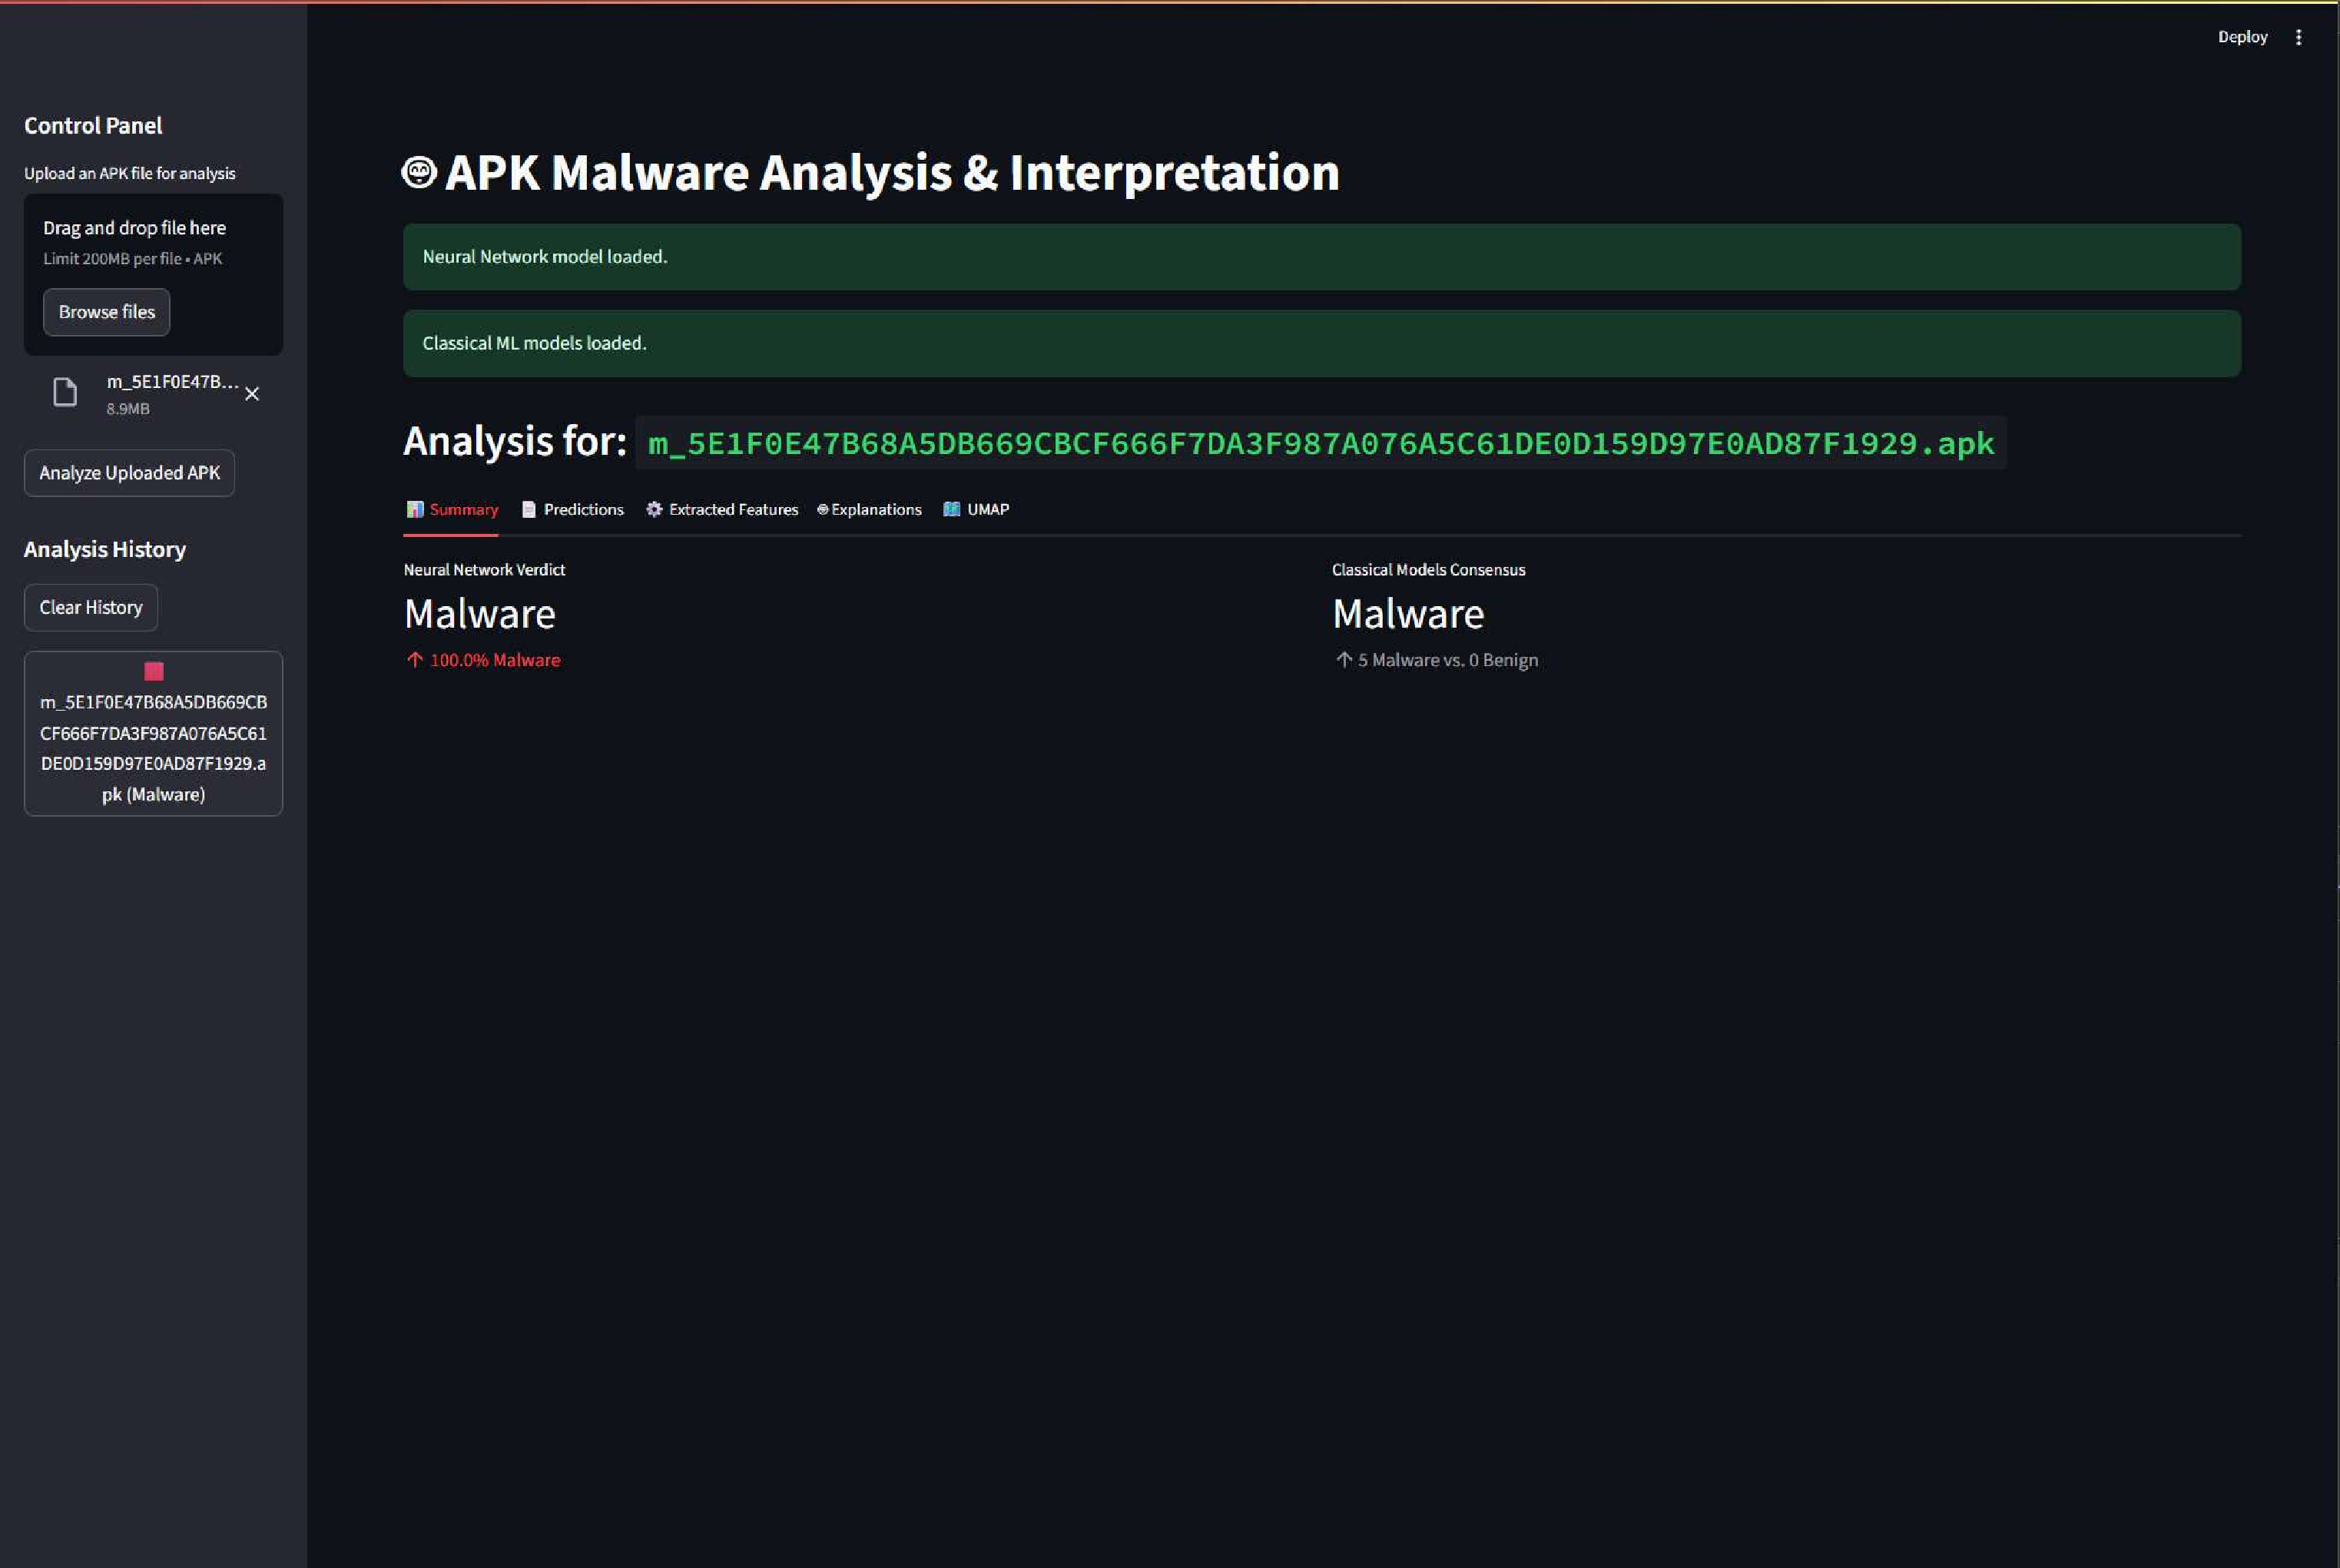
\includegraphics[width=\linewidth]{streamlit_app_main} 
		\caption{Página principal}
		\label{fig:streamlitMain}
	\end{subfigure}\hfill
	\begin{subfigure}{0.5\linewidth}
		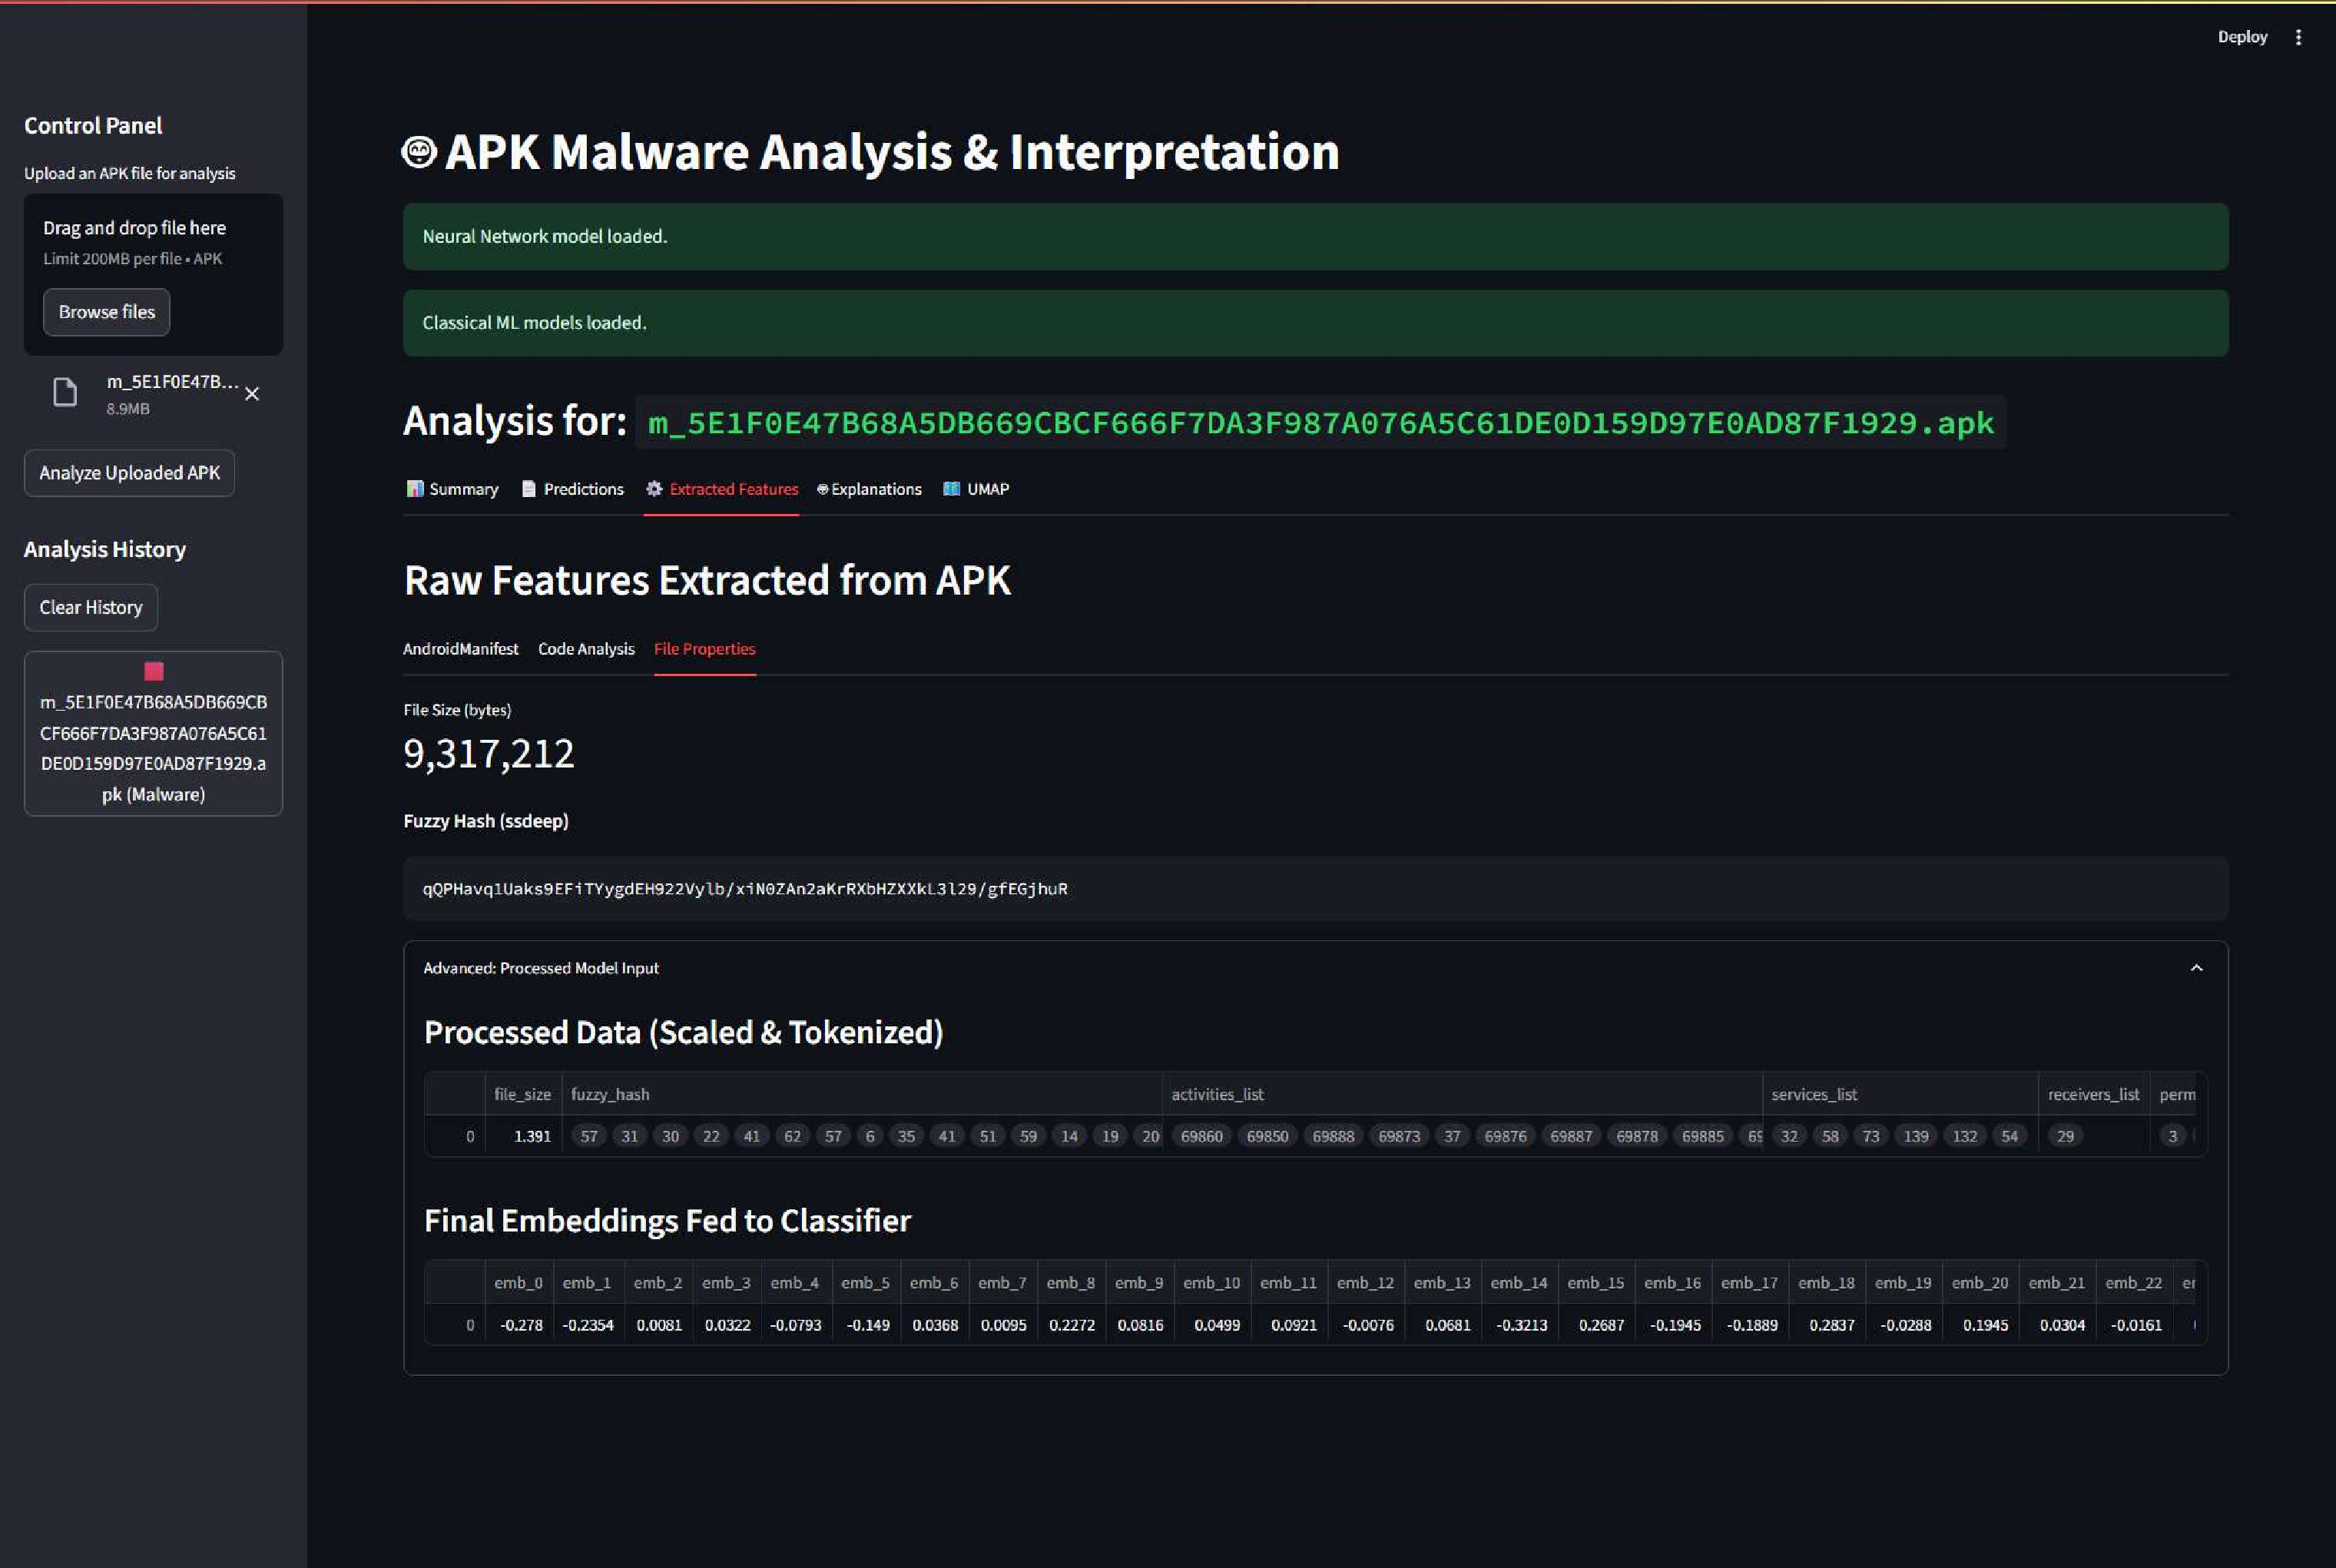
\includegraphics[width=\linewidth]{streamlit_app_extraction_3}
		\caption{Resumen de la extracción}
		\label{fig:streamlitExtraction}
	\end{subfigure}
	
	\begin{subfigure}{0.5\linewidth}
		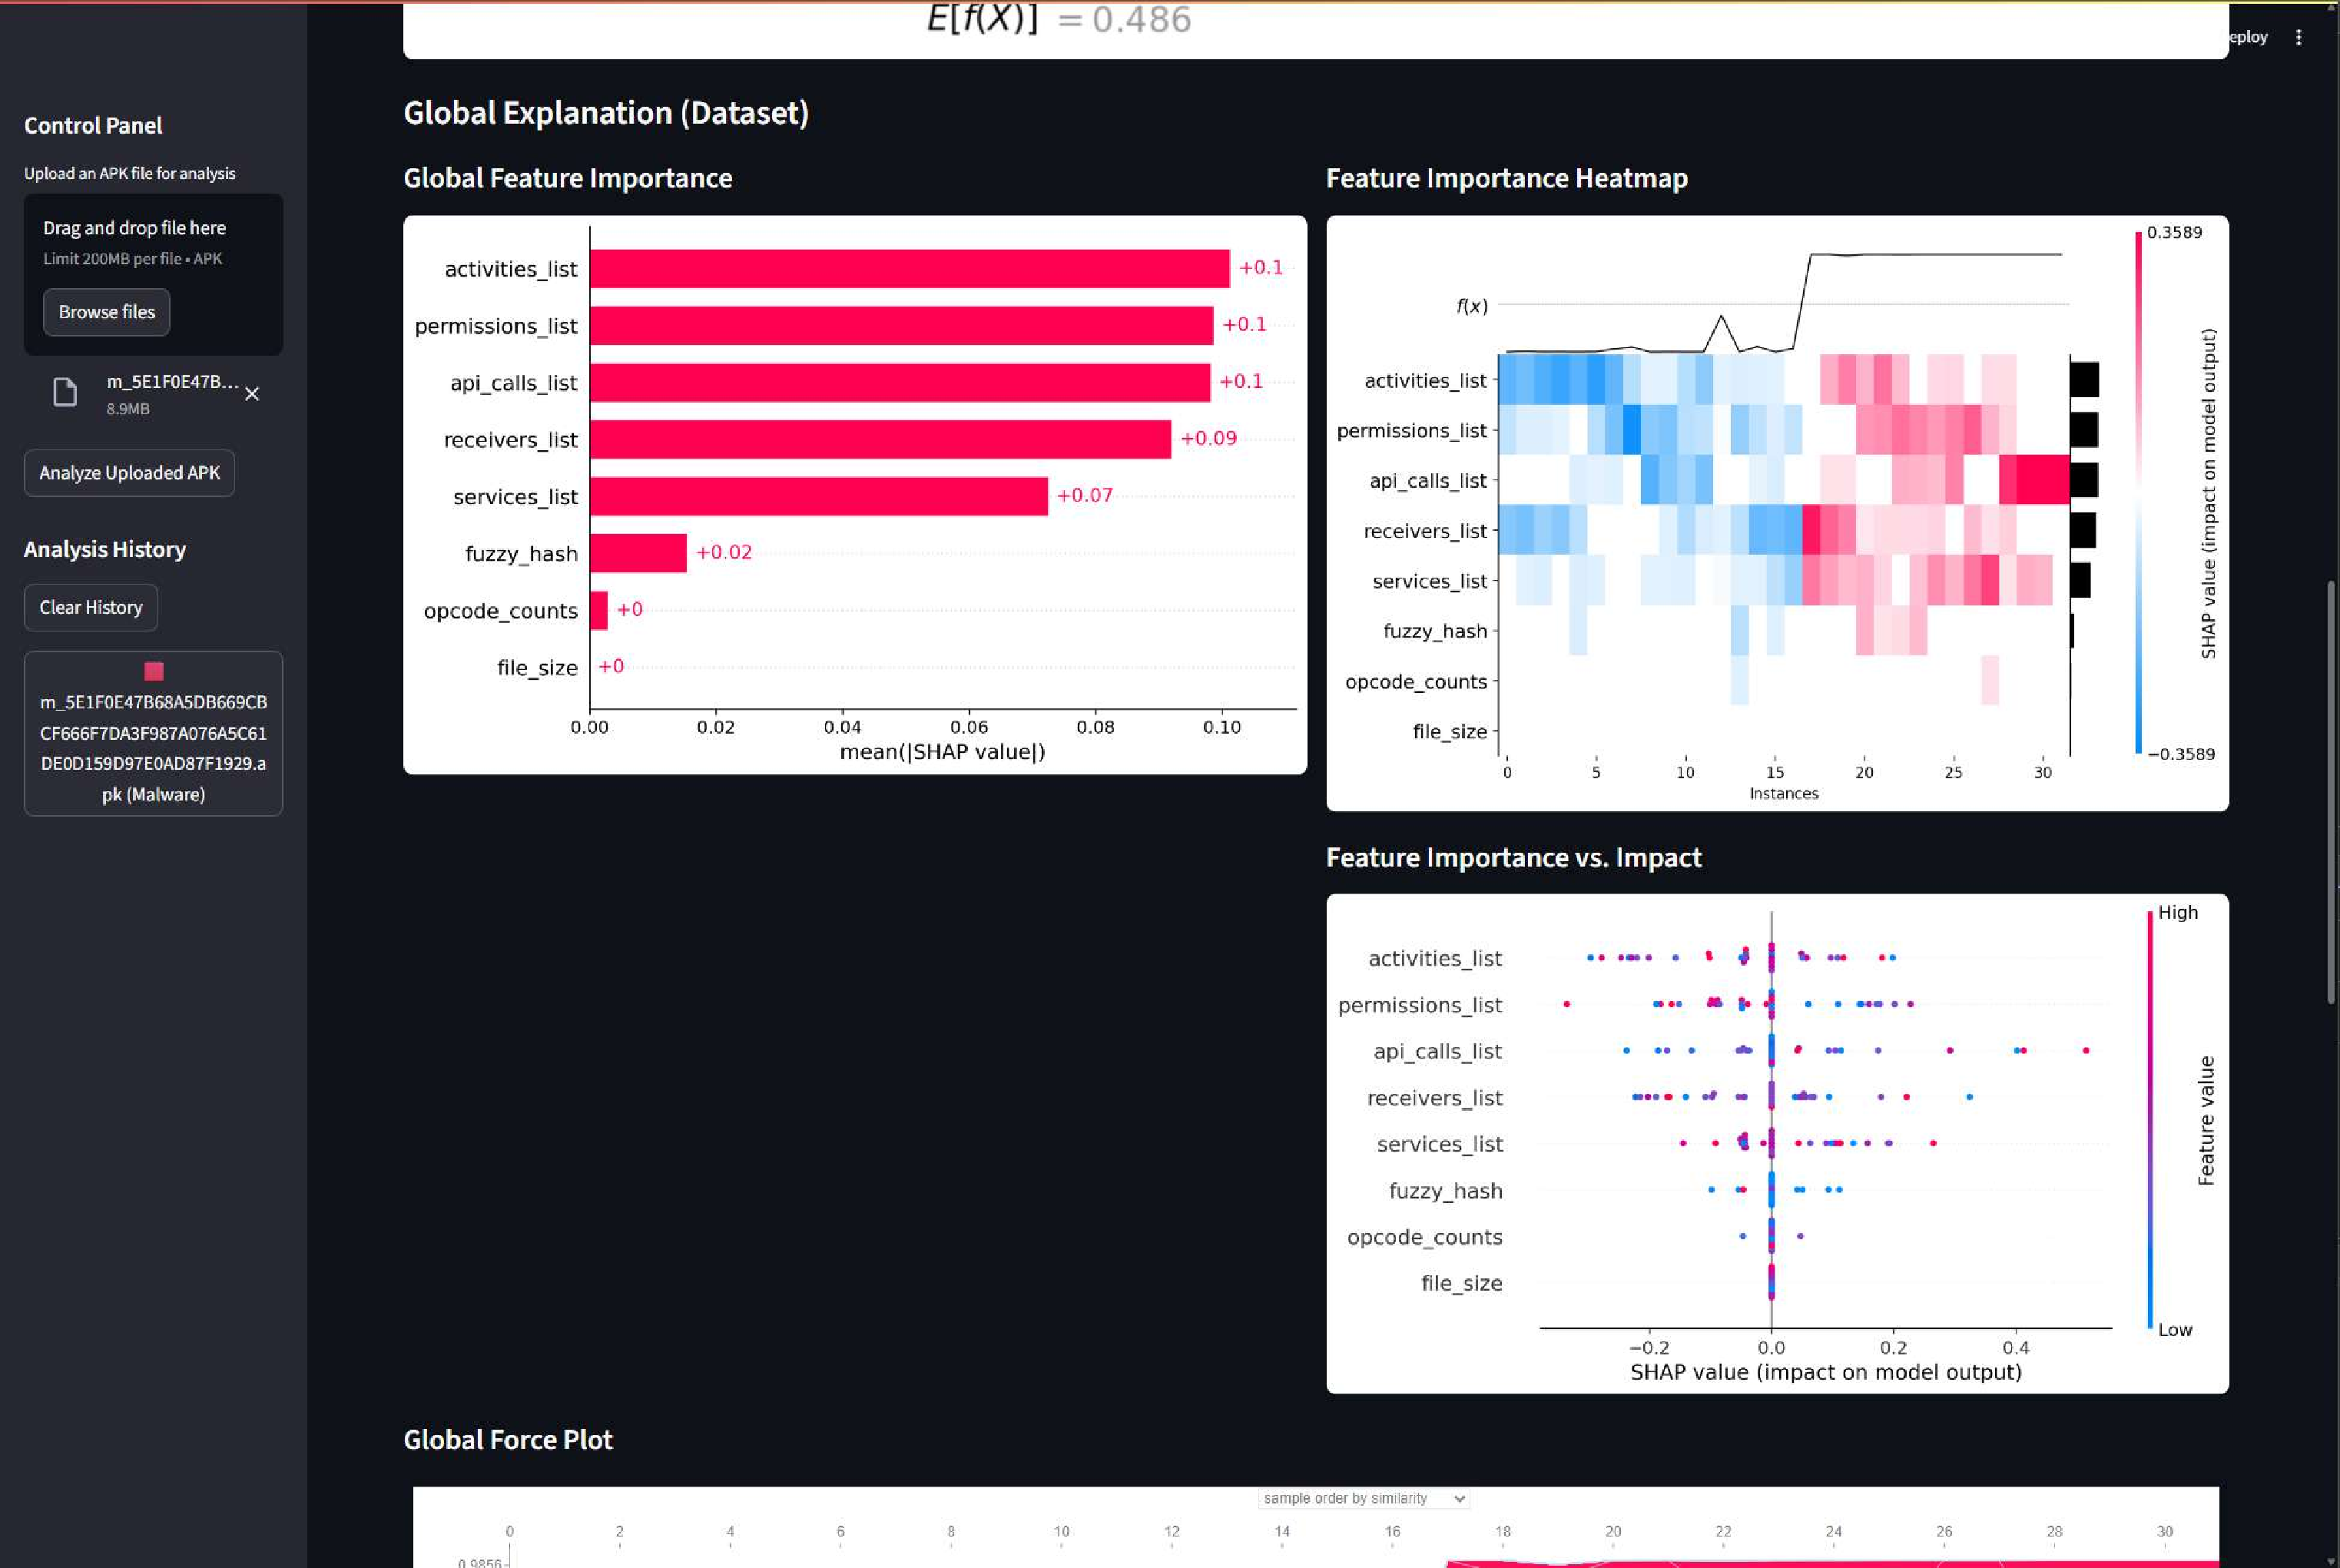
\includegraphics[width=\linewidth]{streamlit_app_shap_2}
		\caption{Análisis de interpretabilidad}
		\label{fig:streamlitSHAP}
	\end{subfigure}\hfill
	\begin{subfigure}{0.5\linewidth}
		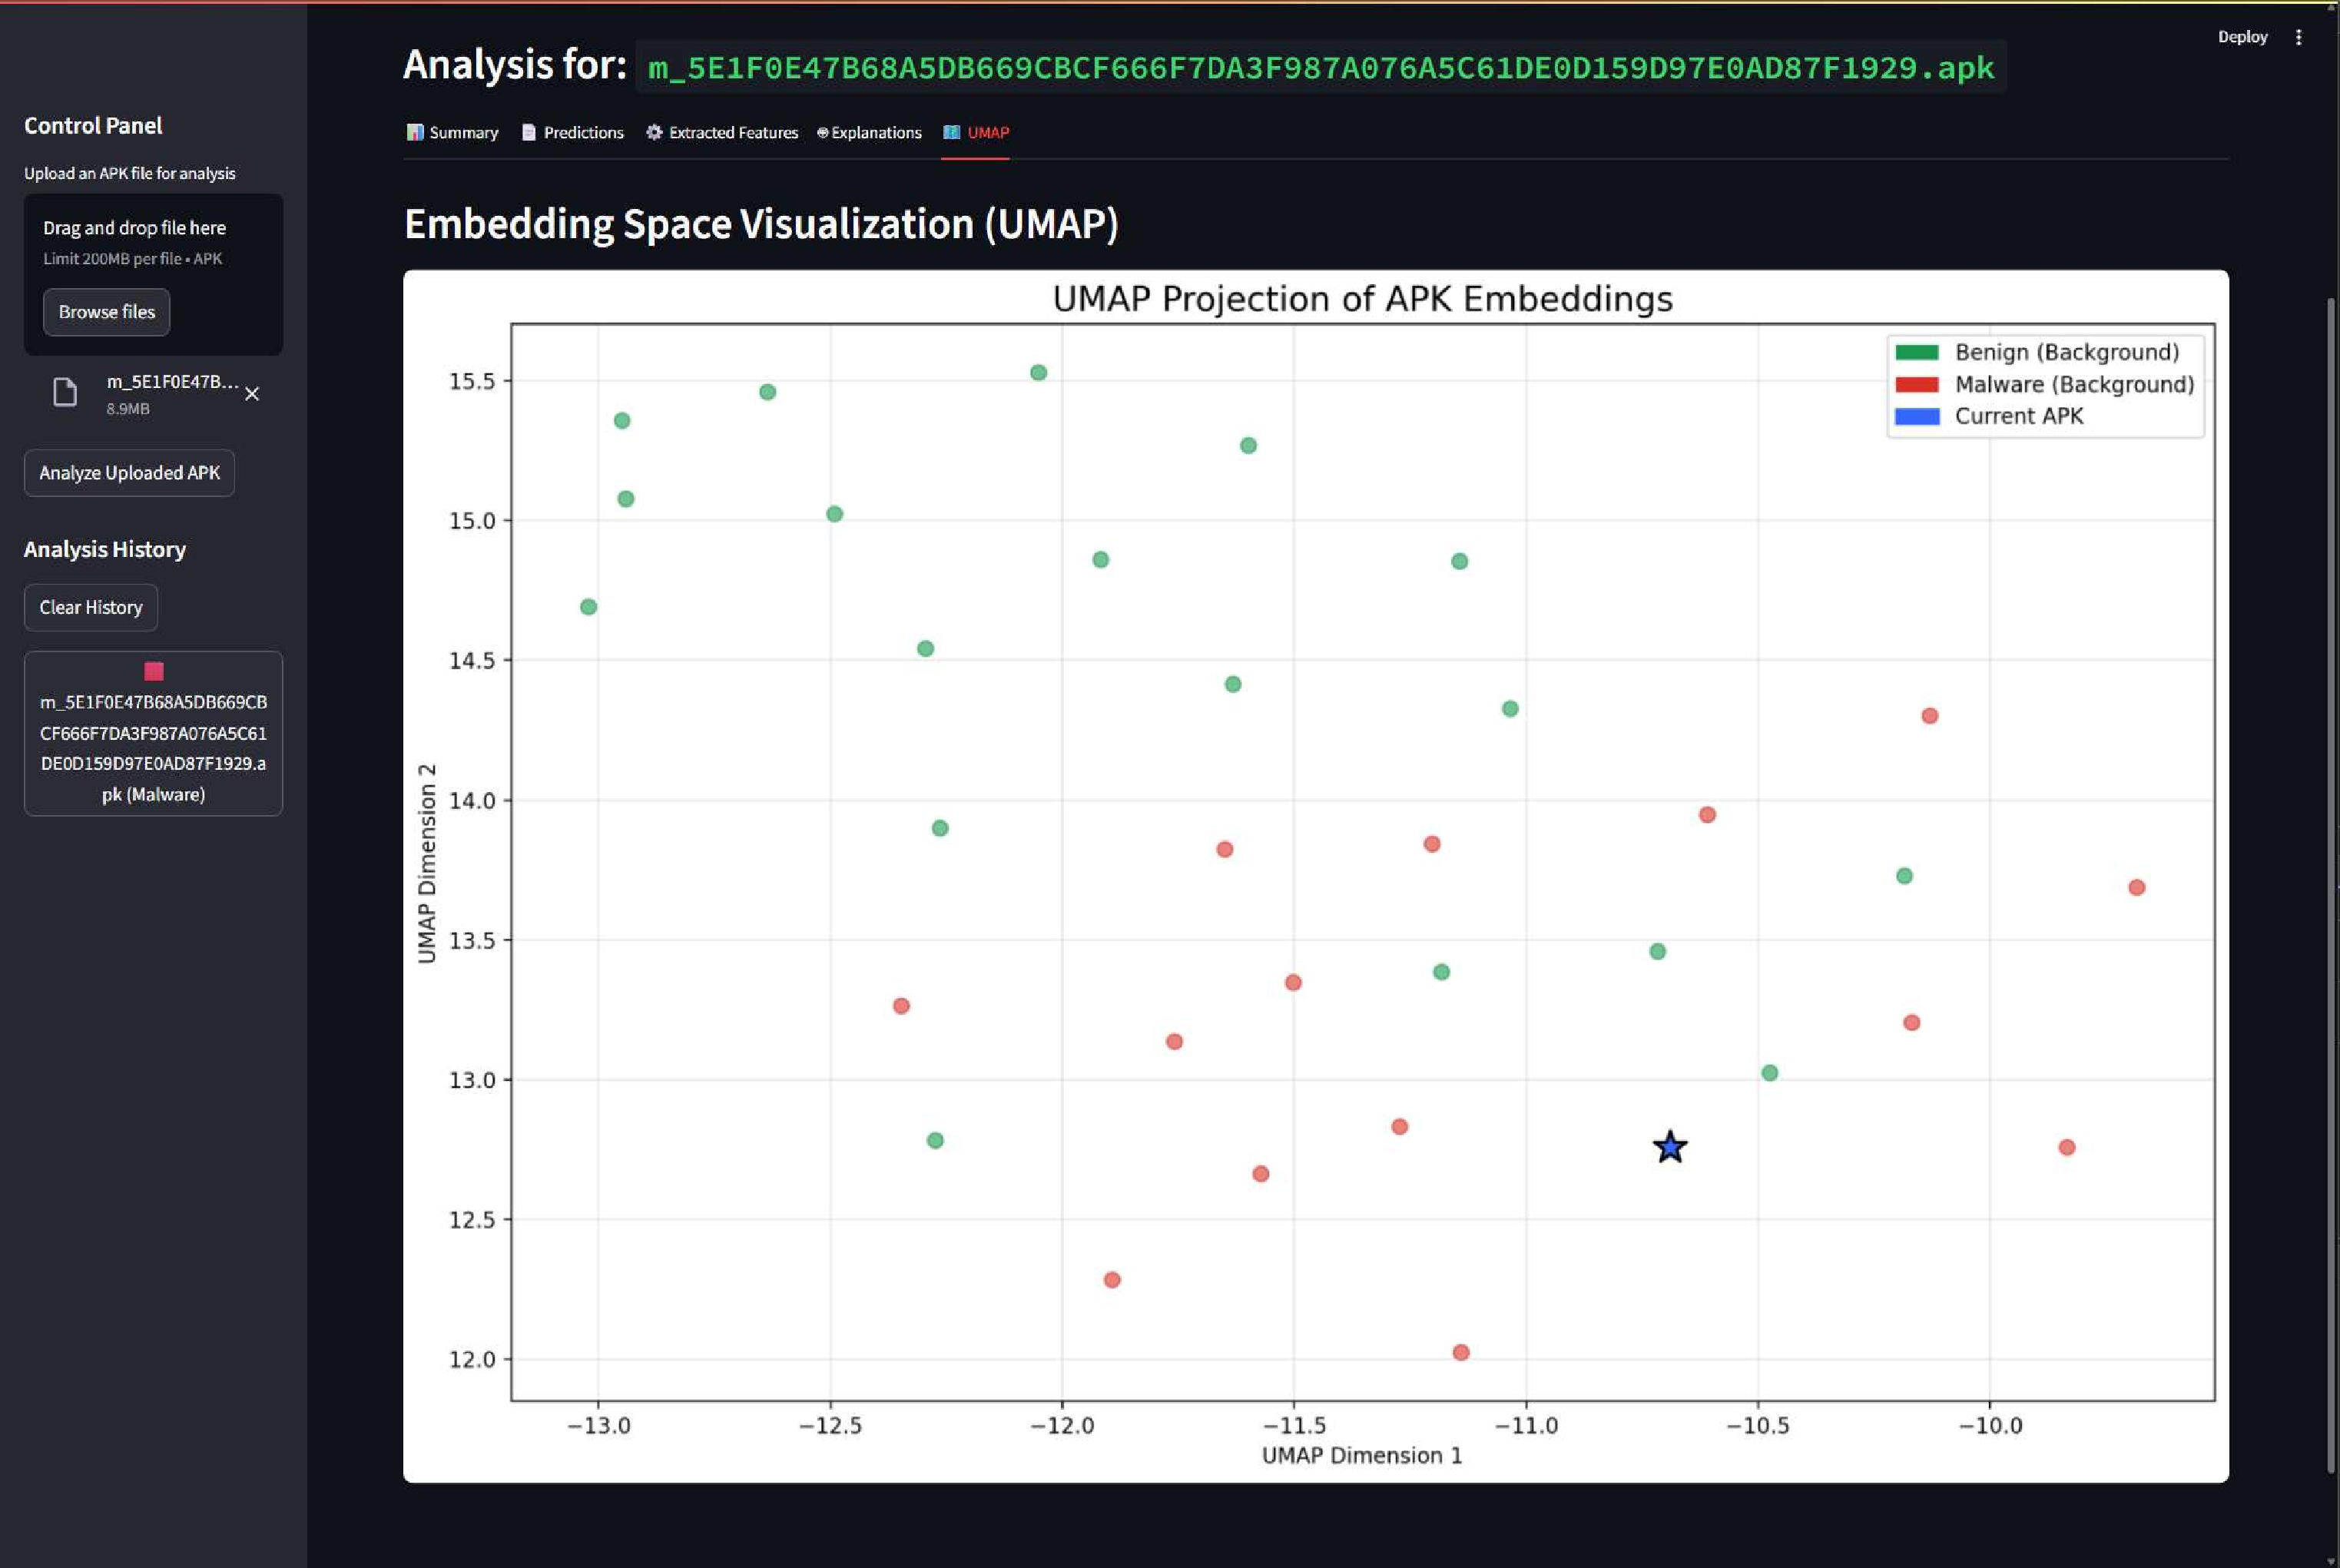
\includegraphics[width=\linewidth]{streamlit_app_umap}
		\caption{Análisis del espacio de \textit{embeddings}}
		\label{fig:streamlitUMAP}
	\end{subfigure}
	
	\caption{Aplicación de demostración del modelo}
	\label{fig:streamlitApp}
\end{figure}


La aplicación se diseñó con una interfaz sencilla y minimalista. Un menú lateral permite al usuario subir un archivo APK y ver un historial de los análisis realizados durante la sesión. La página principal se organiza en pestañas que muestran:

\begin{itemize}
	\item Un resumen de la predicción actual (Figura \ref{fig:streamlitMain}).
	
	\item Los detalles de las características extraídas de la APK (Figura \ref{fig:streamlitExtraction}).
	
	\item Un análisis de interpretabilidad con gráficos de SHAP para el modelo seleccionado (Figura \ref{fig:streamlitSHAP}).
	
	\item La visualización del espacio de \textit{embedding} con UMAP, mostrando dónde se sitúa la aplicación analizada (Figura \ref{fig:streamlitUMAP}).
\end{itemize}

De esta forma, la aplicación no solo da un resultado, sino que también educa al usuario sobre el proceso interno del modelo.

\subsection{\textit{Dockerización} y despliegue}

Para facilitar la prueba y la distribución de la aplicación, se decidió empaquetarla en un contenedor de Docker. Esto permite que cualquier persona con Docker instalado pueda ejecutar la aplicación con un único comando, sin preocuparse por instalar Python o cualquiera de las numerosas dependencias del proyecto. El \texttt{Dockerfile} se encargó de preparar el entorno utilizando Poetry para instalar los paquetes, y de iniciar el servidor de Streamlit, exponiendo el puerto correspondiente.

El despliegue final se realizó en un servidor de la universidad. El proceso consistió en conectarse a la red del centro mediante una VPN, acceder a la máquina remota por SSH, transferir los archivos del proyecto mediante SCP y, finalmente, ejecutar el contenedor de Docker. Esto permitió que la aplicación fuera accesible desde dentro de la red de la universidad\footnote{Disponible en este dirección: \url{http://10.168.168.34:8501/}}, completando así el ciclo de vida del proyecto desde la investigación hasta el despliegue de una herramienta funcional.
